\chapter{Prace nad architekturą i infrastrukturą projektu}
\label{cha:infra}


Niniejszy rozdział zawiera opis prac wykonanych przez autorów w ramach rozwoju architektury i infrastruktury systemu GGSS. Rozdział ten stanowi bezpośrednią kontynuację pracy inżynierskiej autorów, gdzie przygotowane zostały pierwsze wersje rozwijanych w ramach pracy magisterskiej rozwiązań. Przedstawione tu informację dotyczą szerokiego zakresu zagadnień związanych z inżynierią oprogramowania, takich jak: zarządzanie strukturą projektu oraz jego zależnościami, automatyzacja procesów towarzyszących wytwarzaniu oprogramowania czy przygotowanie infrastruktury ułatwiającej testy warstwy sprzętowej systemu. 

\section{Zmiany w architekturze projektu}
Przez zmiany w architekturze projektu autorzy rozumieją stopniowy rozwój rozwiązania przygotowanego w ramach napisanej przez nich pracy inżynierskiej. Wprowadzone po jej zakończeniu modyfikacje to przede wszystkim uproszczenie powstałej hierarchii zależności między poszczególnymi elementami warstwy oprogramowania (rozumianymi zarówno jako repozytoria, jak i biblioteki), uczynienie systemu bardziej przystępnym dla użytkownika (np. poprzez nadanie komponentom nazw dobrze oddających ich przeznaczenie) oraz przygotowanie systemu pozwalającego w prosty sposób odtworzyć kod źródłowy w wersji bez wprowadzonych w ramach pracy magisterskiej modyfikacji (jako rodzaj zabezpieczenia przed skutkami potencjalnych błędów, które mogły zostać wprowadzone do oprogramowania podczas prac nad nim). Znaczna część zmian opisanych w niniejszej części pracy była możliwa do wprowadzenia z uwagi na trwające jednocześnie prace nad kodem źródłowym systemu GGSS i zmiany zachodzące w ich czasie. 


\subsection{Początkowa architektura projektu}
Przeprowadzone przez autorów w ramach pracy inżynierskiej modyfikacje architektury systemu GGSS obejmowały przede wszystkim migrację projektu do systemu kontroli wersji Git, wprowadzenie spójnego nazewnictwa poszczególnych komponentów oraz zastosowanie funkcjonalności submodułów będącej częścią technologii Git do stworzenia hierarchicznej struktury repozytoriów (w odróżnieniu od pierwotnej, płaskiej architektury opartej o katalogi). Celem tych zmian było ułatwienie pracy nad pojedynczymi komponentami projektu oraz uczynienie struktury projektu przyjazną dla użytkownika, co zostało zdaniem autorów osiągnięte. 

Architektura stanowiąca punkt wyjściowy zmian wykonanych w ramach niniejszej pracy przedstawiona została na rysunku \ref{fig:old_structure} (z pominięciem repozytoriów pomocniczych, zawierających np. dokumentację). Projekt składał się więc pierwotnie z 14 repozytoriów zawierających wchodzące w skład oprogramowania systemu GGSS biblioteki, aplikacje i skrypty. Przygotowane w ten sposób rozwiązanie charakteryzowało się jednak pewnymi wadami i ograniczeniami, z których najważniejsze to:
\begin{itemize}
    \item głęboka hierarchia zależności, mająca negatywny wpływ na wydajność działania mechanizmu submodułów
    \item istnienie repozytorium \emph{ggss-misc}, zawierającego (poza szablonami CMake) elementy kodu źródłowego niepasujące do pozostałych bibliotek wchodzących w skład systemu: bazowe klasy wyjątków stosowanych w całym projekcie oraz flagi konfigurujące projekt w zależności od systemu operacyjnego (konieczność zastosowania tego typu zabiegu wynikła wprost z założenia o niemodyfikowaniu kodu źródłowego w czasie tworzenia pracy inżynierskiej)
    \item zachowanie oryginalnych nazw bibliotek i aplikacji, dostosowując je jedynie do przyjętej konwencji. Jedną z bibliotek wchodzących w skład projektu była biblioteka statyczna \emph{handle-lib}, odpowiedzialna za implementację mechanizmu slotów i sygnałów (\textbf{pisownia}), na co, zdaniem autorów, jej nazwa nie wskazuje.
    \item wnioskowanie o zależnościach pomiędzy bibliotekami na podstawie dyrektyw preprocesora \emph{include} zawartych w kodzie źródłowym, a nie wykorzystywanych funkcjonalności, co wynikało z niewielkiego doświadczenia i wiedzy autorów na temat systemu podczas tworzenia pracy inżynierskiej oraz wspomnianego już założenia o niemodyfikowaniu kodu źródłowego.
    \item założenie o tworzeniu oddzielnego repozytorium dla każdej z występujących w projekcie aplikacji, niezależnie od jej rozmiarów, co ostatecznie znacznie skomplikowało powiązania pomiędzy repozytoriami (np. repozytoria \emph{external-caen-n957-demo} oraz \emph{mca-n957} charakteryzują się podobnymi zależnościami i oba zawierają niewielkie aplikacje, których zadaniem jest współpraca z wielokanałowym analizatorem amplitudy CAEN N957 - mogłoby być więc połączone w jedno repozytorium).
    \item brak łatwego sposobu na odtworzenie pierwotnej postaci kodu źródłowego - mechanizm ten nie był potrzebny na etapie pracy inżynierskiej, ponieważ nie dokonywano wtedy modyfikacji we wspomnianym kodzie.
\end{itemize}

\begin{landscape}

\begin{figure}[H]
\centering
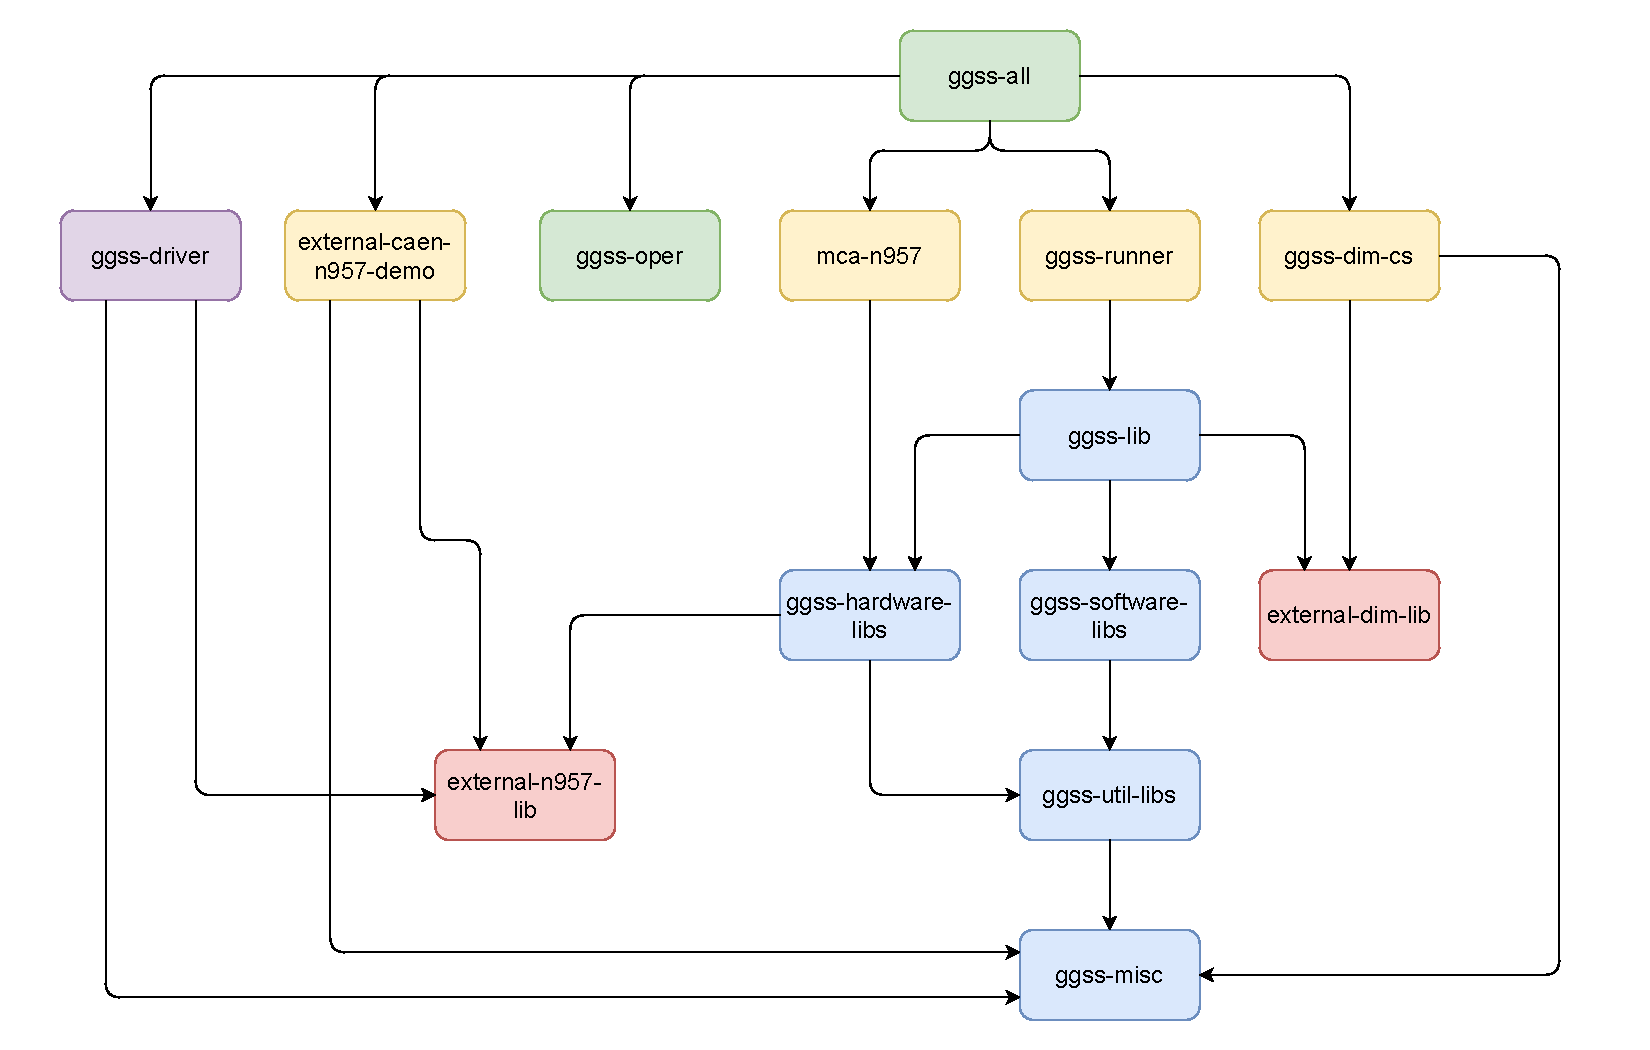
\includegraphics[width=1.4\textwidth]{components/infra_images/old_structure.pdf}
\caption{}
\label{fig:old_structure}
\end{figure}

\end{landscape}

\subsection{Uproszczenie architektury projektu}
Pierwszym podjętym przez autorów działaniem mającym na celu modyfikację struktury projektu była próba jej uproszczenia poprzez analizę zależności wewnętrzych systemu (tzn. zależności pomiędzy poszczególnymi bibliotekami). Należy tutaj zwrócić uwagę, że prac tych nie wykonywano przez pierwsze pół roku od rozpoczęcia przez autorów studiów magisterskich - skupienie się na użytkowaniu stworzonej architektury pozwoliło autorom zarówno na zapoznanie się lepiej z projektem, jak również na samodzielną obserwację jej zalet i wad. 

W celu zrozumienia wprowadzonych w projekcie zmian, konieczne jest zrozumienie toku rozumowania, jakim posługiwali się autorzy pracy podczas tworzenia oryginalnej struktury projektu - dotyczy to przede wszystkim repozytoriów \emph{ggss-lib}, \emph{ggss-software-libs}, \emph{ggss-hardware-libs}, \emph{ggss-util-libs} oraz \emph{ggss-misc}. Ich rola w projekcie prezentuje się następująco:
\begin{itemize}
    \item \emph{ggss-hardware-libs} - przechowywanie bibliotek odpowiedzialnych za obsługę urządzeń wchodzących w skład warstwy sprzętowej systemu GGSS. W pierwotnej wersji projektu były to następujące biblioteki:
    \begin{itemize}
        \item \emph{caenhv-lib} oraz \emph{caenn1470-lib} - odpowiedzialne za komunikację z zasilaczami wysokiego napięcia CAEN N1470
        \item \emph{mca-lib} oraz \emph{ortecmcb-lib} - odpowiedzialne za obsługę wielokanałowego analizatora amplitudy CAEN N957
        \item \emph{usbrm-lib} - odpowiedzialna za obsługę multipleksera sygnałów analogowych
    \end{itemize}
    \item \emph{ggss-software-libs} - przechowywanie bibliotek odpowiedzialnych za implementację wykorzystywanych przez system algorytmów i struktur danych związanych ściśle z warstwą oprogramowania (tzn. nie mających związku z warstwą sprzętową). W pierwotnej wersji projektu były to następujące biblioteki:
    \begin{itemize}
        \item \emph{xml-lib}
        \item \emph{fifo-lib}
        \item \emph{fit-lib}
        \item \emph{daemon-lib}
    \end{itemize}
    \item \emph{ggss-util-libs} - przechowywanie bibliotek, od których zależne są zarówno komponenty odpowiedzialne za obsługę warstwy sprzętowej projektu, jak i związane wyłącznie z warstwą oprogramowania. Innymi słowy, są to biblioteki nie mogące znaleźć się w żadnym z dwóch wymienionych powyżej repozytoriów. W pierwotnej wersji projektu były to:
    \begin{itemize}
        \item \emph{log-lib}
        \item \emph{utils-lib}
        \item \emph{handle-lib}
        \item \emph{thread-lib}
    \end{itemize}
    \item \emph{ggss-misc} - 
    \item \emph{ggss-lib} - przechowywanie kodu źródłowego zawierającego główną logikę systemu GGSS
\end{itemize}

Prace nad kodem źródłowym projektu pozwoliły autorom zaobserwować, iż pewna część występujących w nim dyrektyw preprocesora \emph{include} nie oddaje w poprawny sposób faktycznej struktury zależności między bibliotekami. Najważniejszy przykład stanowi łańcuch zależności występujących pomiędzy biblioteką \emph{ggss-lib}, a bibliotekami \emph{caenhv-lib} oraz \emph{thread-lib}. W oryginalnej wersji projektu zależności między wymienionymi komponentami prezentowały się tak, jak na rysunku \ref{fig:dependency_problem_old}, tzn. bibliteka \emph{ggss-lib} zależna była od biblioteki \emph{caenhv-lib}, która natomiast zawierała dyrektywę \emph{include} dołączającą plik nagłówkowy z biblioteki \emph{thread-lib}. 


\savebox{\mybox}{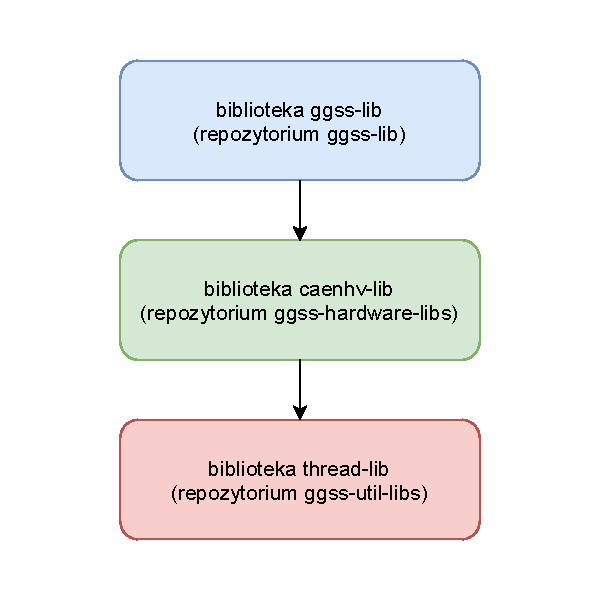
\includegraphics[width=0.40\textwidth]{components/infra_images/dependency_problem_old.pdf}}

\begin{figure}[H]
\centering
\begin{subfigure}[t]{0.40\textwidth}
\centering
\usebox{\mybox}
\caption{Test}
\label{fig:dependency_problem_old}
\end{subfigure}
\hfill
\begin{subfigure}[t]{0.55\textwidth}
\centering
\vbox to \ht\mybox{%
    \vfill
    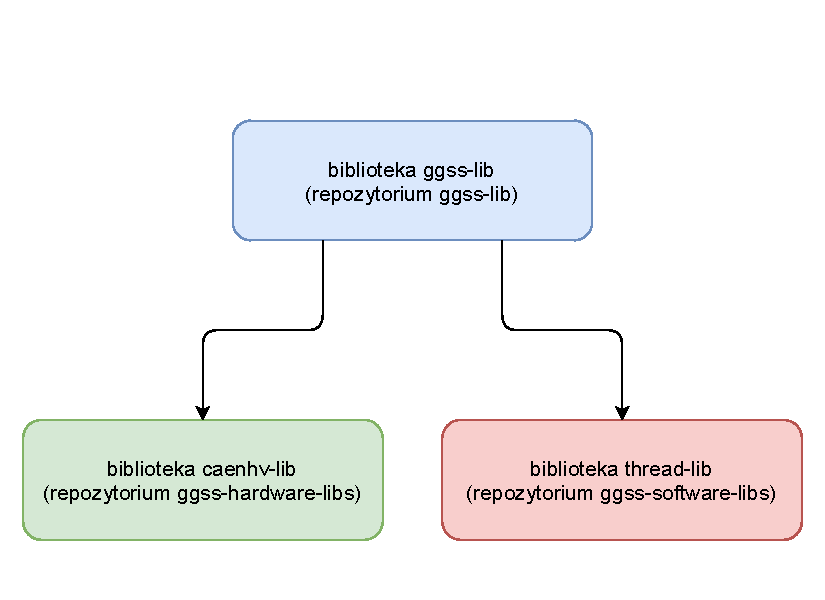
\includegraphics[width=\textwidth]{components/infra_images/dependency_problem_solution.pdf}
    \vfill
}
\caption{Test}
\label{fig:dependency_problem_solved}
\end{subfigure}

\caption{Test}
\end{figure}

W rzeczywistości biblioteka \emph{caenhv-lib} nie wykorzystywała zawartości wspomnianego pliku nagłówkowego - pełniła jedynie formę swego rodzaju pośrednika, udostępniając znajdujące się tam klasy bibliotece \emph{ggss-lib}. Przeniesienie dyrektywy \emph{include} do biblioteki \emph{ggss-lib} spowodowało, iż żadna z bibliotek wchodzących w skład repozytorium \emph{ggss-hardware-libs} nie zawierała zależności do biblioteki \emph{thread-lib}. Rozwiązanie to pozwoliło dokonać migracji tejże biblioteki, wraz z wykorzystywaną przez nią biblioteką \emph{handle-lib}, do repozytorium \emph{ggss-software-libs}, redukując tym samym liczbę bibliotek znajdujących się w repozytorium \emph{ggss-util-libs}. Rysunek \ref{fig:dependency_problem_solved} przedstawia w sposób schematyczny strukturę otrzymanego rozwiązania.

W związku z opisanymi powyżej zmianami ilość kodu źródłowego znajdującego się w repozytorium \emph{ggss-util-libs} znacznie spadła - pozostałe tam biblioteki \emph{log-lib} oraz \emph{utils-lib} charakteryzowały się niewielkim rozmiarem. Spowodowało to, iż jednoczesne istnienie modułów \emph{ggss-misc} oraz \emph{ggss-util-libs} (po wprowadzonych zmianach spełniających tą samą rolę przechowywania niewielkiej liczby komponentów wykorzystywanych przez wiele modułów projektu GGSS) przestało być uzasadnione. Kolejny etap wykonanych prac stanowiło więc przeprowadzenie integracji tychże repozytoriów - w tym celu zdecydowano się na likwidację modułu \emph{ggss-misc} po wcześniejszym przeniesieniu jego zawartości do \emph{ggss-util-libs}.

Migracja znajdujących się w repozytorium \emph{ggss-misc} plików \emph{.cmake} (modułów wykorzystywanych przez infrastrukturę budowania projektu) wymagała, poza wykonaniem trywialnej czynności przeniesienia katalogu, aktualizacji (na poziomie całego projektu) ścieżek wskazujących lokalizację tychże plików. Działanie to było konieczne, ponieważ narzędzie CMake wymaga od programisty, by wyspecyfikował on lokalizację modułów \emph{.cmake} dołączanych do projektu (np. za pomocą komendy \lstinline{include()}) poprzez dodanie ścieżki z ich lokalizacją do listy \lstinline{CMAKE_MODULE_PATH} (przykład wykorzystania tejże listy przedstawiony został na listingu \textbf{listing}). Oznaczało to więc konieczność wykonania, w każdym module wykorzystującym pliki \emph{.cmake}, zmiany wspomnianej ścieżki tak, by wskazywała na katalog \emph{cmake-templates} w repozytorium \emph{ggss-util-libs}.

Poza wspomnianymi plikami \emph{.cmake} w repozytorium \emph{ggss-misc} znajdował się katalog \emph{include}, zawierający trzy pliki nagłówkowe z kodem napisanym w języku C++:
\begin{itemize}
    \item pliki \lstinline{ggssExceptions.h} oraz \lstinline{HardwareException.h} zawierające klasy bazowe wyjątków wykorzystywanych w całym projekcie GGSS
    \item plik \lstinline{CompatibilityFlags.h}, zawierający flagi konfigurujące projekt w zależności od platformy docelowej (Windows lub Linux)
\end{itemize}
Pliki te nie wchodziły oryginalnie w skład żadnej z bibliotek projektu GGSS, nie mogły zostać do nich również dodane przez autorów podczas przygotowywania pracy inżynierskiej, ponieważ wymagałoby to modyfikacji kodu źródłowego systemu. Podczas przeprowadzanej w ramach niniejszej pracy migracji tych plików do repozytorium \emph{ggss-util-libs} zdecydowano się na likwidację katalogu \emph{include} i rozdysponowanie jego zawartości do istniejących lub nowych bibliotek. Plik \lstinline{CompatibilityFlags.h} przeniesiony został więc do biblioteki \emph{utils-lib}, natomiast na potrzebę dwóch pozostałych nagłówków przygotowana została nowa biblioteka \emph{exceptions-lib}. 

Finalna struktura repozytorium \emph{ggss-util-libs} przedstawiona została na listingu \textbf{listing}. Poza wspomnianymi do tej pory zmianami nowość stanowi katalog \lstinline{doxygen-config}, zawierający prosty plik konfigurujący działanie narzędzia Doxygen \textbf{cytat} służącego do generowania dokumentacji programów napisanych w języku C++. Rozszerzenie projektu o możliwość generowania dokumentacji zostanie jednak opisane szczegółowo w dalszej części pracy (sekcja \textbf{dodac referencje do sekcji}).


Poza wspomnianymi do tej pory repozytoriami zmianami objęte zostały ponadto moduły przechowujące aplikacje służące do testowania i obsługi urządzeń elektronicznych wchodzących w skład warstwy sprzętowej systemu GGSS. Motywacją do wprowadzenia modyfikacji była konieczność rozbudowy projektu o kolejne tego typu aplikacje (co zostanie szerzej opisane w sekcji \textbf{sekcja}) - tworzenie dla każdej z nich osobnego repozytorium znacząco komplikowałoby strukturę projektu. Zdecydowano zatem, iż repozytoria \emph{mca-n957} oraz \emph{external-caen-n957-demo} zostaną dołączone do nowo powstałego repozytorium \emph{ggss-hardware-service-apps}, grupującego niewielkie programy służące do operowania na urządzeniach.


% TODO: moze wspomniec o koniecznosci zachowania historii i jak zostało to zrobione???

Poza zmniejszeniem progu wejścia do projektu poprzez uczynienie jego struktury prostszą, opisane do tej pory zmiany korzystnie wpłynęły na działanie mechanizmu submodułów systemu Git, na którym oparty został proces zarządzania zależnościami między repozytoriami w projekcie. Redukcja liczby repozytoriów i powiązań między nimi oraz zmniejszenie głębokości drzewa zależności (poprzez likwidację repozytorium \emph{ggss-misc}) miało pozytywny wpływ na wydajność systemu zarządzającego architekturą projektu. 



\subsection{Dodanie możliwości odtworzenia pierwotnej wersji kodu źródłowego}
% branche legacy, dokumentacja

\subsection{Pomniejsze zmiany}
Poza do tej pory opisanymi, wykonanych zostało kilka pomniejszych modyfikacji mających na celu szeroko pojętą poprawę jakości struktury projektu. Przeprowadzone prace obejmują bogaty zakres wprowadzonych zmian, nie jest więc możliwe zamieszczenie w niniejszej pracy dokładnego opisu każdej z nich. Poniżej krotko opisane zostały więc trzy wybrane przez autorów modyfikacje, charakteryzujące się różnym poziomem skomplikowania, ale operujące na poziomie pojedynczych repozytoriów. 

\subsubsection{Likwidacja repozytorium \emph{ggss-oper}}
Jednym z repozytoriów wprowadzonych przez autorów w ramach wykonywania pracy inżynierskiej był moduł \emph{ggss-oper}, zawierający skrypty oraz pliki konfiguracyjne stanowiące znaczną część infrastruktury przeznaczonej do użytkowania wraz z oprogramowaniem GGSS na maszynie docelowej. Zawartość tego repozytorium, nie stanowiąca wkładu wniesionego przez autorów niniejszej pracy w system, obejmowała m.in.: 
\begin{itemize}
    \item pierwsze wersje skryptów służących do przeprowadzania testów urządzeń wchodzących w skład warstwy sprzętowej projektu (napisane z wykorzystaniem języka Python)
    \item skrypty zarządzające stanem środowiska docelowego (np. ustawiające wymagane zmienne środowiskowe)
    \item skrypty zarządzające oprogramowaniem systemu GGSS, np. \emph{ggss\_monitor.sh} pozwalający na uruchamianie, zatrzymywanie oraz sprawdzanie stanu aplikacji \emph{ggss-runner}
\end{itemize}
Wraz z postępami prac nad projektem, część z wymienionej powyżej zawartości zastąpiona została przez autorów pracy rozwiązaniami alternatywnymi (np. skrypty służące do przeprowadzania operacji na urządzeniach zastąpione zostały aplikacjami napisanymi w języku C++), pozostałe przeniesione zostały natomiast do repozytorium \emph{ggss-all}. Ostatecznie moduł został więc zlikwidowany.


\subsubsection{Utworzenie biblioteki \emph{asyncserial-lib}}
Podczas prac nad kodem źródłowym bibliotek statycznych wchodzących w skład repozytorium \emph{ggss-hardware-libs} zaobserwowano, że w katalogach bibliotek \emph{usbrm-lib} oraz \emph{caenn1470-lib} zamieszczony został, poza właściwym dla nich kodem źródłowym, zestaw plików zawierających implementację asynchronicznej komunikacji z urządzeniami za pomocą interfejsu szeregowego. Ponieważ znalezione w obu przypadkach pliki nie różniły się od siebie, i jednocześnie stanowiły niezbędny element wspomnianych komponentów systemu (zawierały kluczową dla działania projektu funkcjonalność), zdecydowano o utworzeniu nowej biblioteki zawierającej omawiane pliki. Biblioteka nazwana została, zgodnie ze swoim przeznaczeniem, \emph{asyncserial-lib} i weszła w skład repozytorium \emph{ggss-hardware-libs}.


\subsubsection{Zmiana nazwy biblioteki \emph{handle-lib}}
Jedną z bibliotek będących częścią systemu GGSS była biblioteka \emph{handle-lib}, odpowiedzialna za implementację mechanizmu slotów i sygnałów \textbf{napisac moze co to}. Oryginalnie biblioteka ta znajdowała się w repozytorium \emph{ggss-util-libs}, jednak wraz z postępem prac przeniesiona została, wraz z biblioteką \emph{thread-lib}, do repozytorium \emph{ggss-software-libs} (powód tej migracji opisany został w sekcji \textbf{podaj sekcje} niniejszej pracy). Nazwa biblioteki nie pozwalała użytkowniki domyślić się, jakie jest jej zastosowanie - z tego powodu zdecydowano się wprowadzić nową nazwę: \emph{sigslot-lib} (od angielskiego \emph{signals and slots}).


\subsection{Podsumowanie: ostateczna struktura projektu}





\section{Automatyzacja pracy z submodułami}
\section{Rozwój systemu budowania projektu}
\section{Automatyzacja i centralizacja wersjonowania projektu}
\section{Pakietowanie i rozlokowanie projektu}
\section{Rozwój infrastruktury do testowania warstwy sprzętowej}

